\section{Filter-Theorie}
\subsection{Normierung}
HP und TF sind auf Grenzfrequenz des Durchlassbereiches $\omega_D$, also $\omega_r = \omega_D$ normiert. Bei BP und BS sind Mittelfrequenz $\omega_r = \omega_D$. Zur \textbf{Entnormierung} wird in der normierten Funktion $S$ durch $\frac{s}{\omega_r}$ ersetzt.
\begin{align*}
	S = \frac{s}{\omega_r} \qquad \Omega = \frac{\omega}{\omega_r} \qquad \sigma' = \frac{\sigma}{\omega_r}
\end{align*}

\subsection{Approximation}
Alle Approximationen müssen Stempel einhalten. Hier ein Beispiel für einen TP-Filter: \script{295}
\begin{center}
	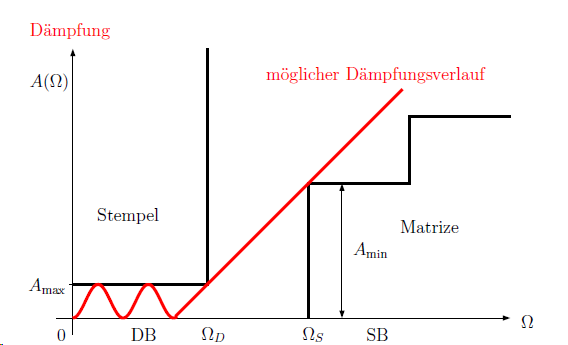
\includegraphics[width=0.5\columnwidth]{Images/tp_matrize}
\end{center}

\subsubsection{kritisch-gedämpfte Filter}\script{299}
Das kritisch-gedämpfte Filter n. Ordnung ist:
\[
	H(s) = \frac{1}{\left(1 + \frac{s}{\omega_c}\right)^n}
\]
Wobei $\omega_c$ den 3dB-Punkt jedes der n Teilfilter bezeichnet. Will man bei der Kreisfrequenz $\omega_D$ eine Dämpfung von $\alpha$ dB haben, so muss $\omega_c$ wie folgt gewählt werden
\[
\omega_c = \frac{\omega_D}{\sqrt{10^{\frac{\alpha}{10\cdot n}}-1}}
\]
3dB Filter mit n. Ordnung kann auf \script{397} gefunden werden.
\begin{center}
	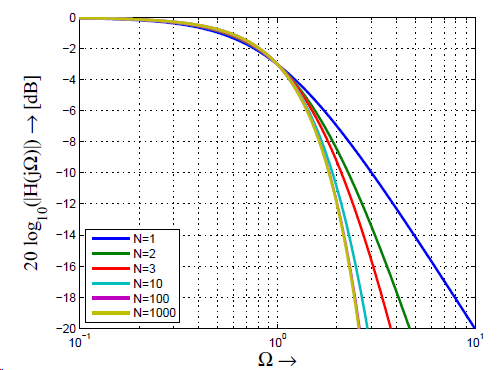
\includegraphics[width=0.6\columnwidth]{Images/kritisch}
\end{center}
\noindent\textbf{Eigenschaften}:
\begin{itemize}[nosep]
	\item n-facher Pol auf negativer $\sigma$-Achse
	\item Impuls- und Sprungantwort kann nicht oszillieren
	\item Allpolfilter: Pole nur auf negativer $\sigma$-Achse
	\item Bei $\Sigma=1$ eine Dämpfung von 3dB
\end{itemize}

\subsubsection{Butterworth}
Der Butterworth Filter für n. Ordnung. Ordnung durch Nomogramm oder mit Formel \script{309} (7.5) bestimmen.
\[
\left|H(j\Omega)\right| = \frac{1}{\sqrt{1 + \Omega^{2n}}}
\]
3dB Filter mit n. Ordnung kann auf \script{399} gefunden werden.
\begin{center}
	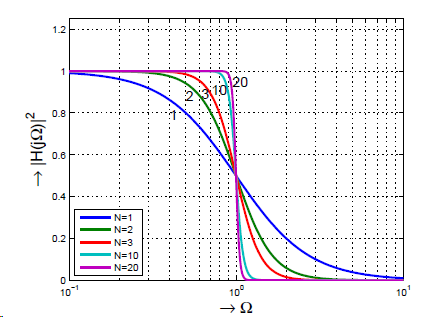
\includegraphics[width=0.6\columnwidth]{Images/butterworth}
\end{center}
\noindent\textbf{Eigenschaften}:
\begin{itemize}[nosep]
	\item Sämtliche Nullstellen im Ursprung
	\item Pole liegen auf Einheitskreis mit Abstand $\pi/n$
	\item Allpolfilter, wobei alle Pole auf einer Ellipse liegen
\end{itemize}

\subsubsection{Tschebyscheff}
Chebyshev Filter mit n. Ordnung, wobei $e=\sqrt{10^{A_{max}/10}-1}$ den Rippelfaktor bestimmt:
\[
\left|H(j\Omega)\right| = \frac{1}{\sqrt{1+ e^2C_n^2(\Omega)}}
\]
\textbf{Hinweis:} UTF von Filter mit Tabelle auf \script{401}~\\
\begin{center}
	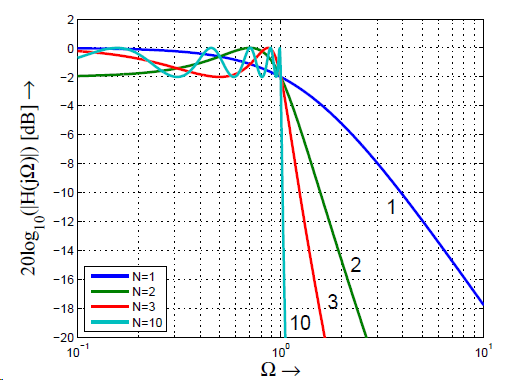
\includegraphics[width=0.6\columnwidth]{Images/tschebyscheff}
\end{center}
\noindent\textbf{Eigenschaften}
\begin{itemize}[nosep]
	\item Nullstellen im Durchlassbereich verteilt
	\item Rippel von $e$ im Durchlassbereich
	\item Allpolfilter (Tscheby. II ist \textbf{kein} Allpolfilter)
\end{itemize}

\subsubsection{Cauer}
Cauer Filter mit n. Ordnung, wobei $e=\sqrt{10^{A_{max}/10}-1}$ den Rippelfaktor bestimmt:
\[
\left|H(j\Omega)\right| = \frac{1}{\sqrt{1+ e^2R_n^2(\Omega)}}
\]
\begin{center}
	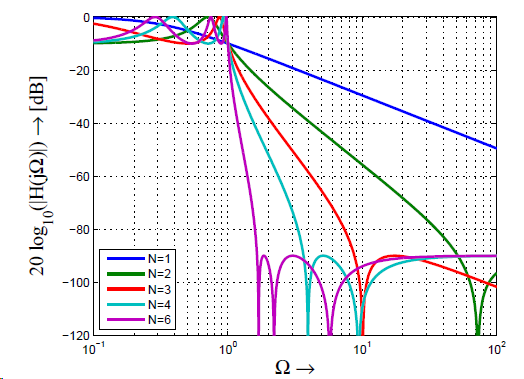
\includegraphics[width=0.6\columnwidth]{Images/cauer}
\end{center}
\noindent\textbf{Eigenschaften}
\begin{itemize}[nosep]
	\item Rippel im DB von $\pm1$
	\item Rippel im SB von $L$
	\item Steiler Übergang von SB zu DB
	\item kein Allpolfilter
\end{itemize}

\subsubsection{Bessel}
\script{329}

\textbf{Hinweis:} UTF von Filter mit Tabelle auf \script{405}~\\
\begin{center}
	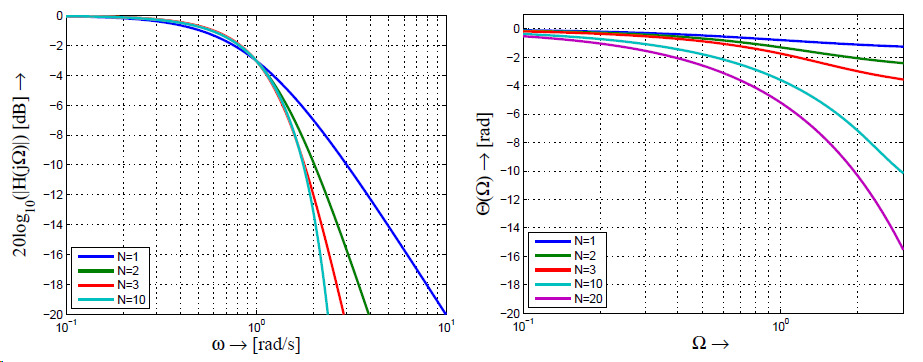
\includegraphics[width=0.8\columnwidth]{Images/bessel}
\end{center}
\noindent\textbf{Eigenschaften}
\begin{enumerate}[nosep]
	\item Möglichst linearer Phasengang, konstante Gruppenlaufzeit
	\item immer asymptotisch stabil
\end{enumerate}

\subsection{Nomogramm}
\script{393} Mittels Stempel und Matrix können die Ordnung von Filtern durch das Nomogramm berechnet werden. Nach folgenden Punkten kann $P_5$ für den nächst höheren gelegene Kurve ($n$) gefunden werden.
\begin{center}
	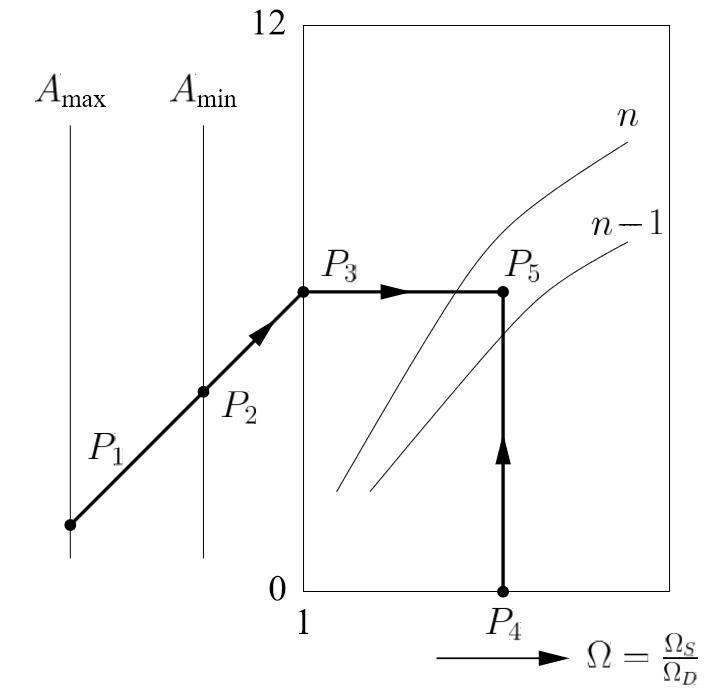
\includegraphics[width=0.6\columnwidth]{Images/nomogramm}
\end{center}
Für Gleichungen siehe \script{394}

\subsection{Transformation}
Die Transformation von TP zu anderen Filtern wird in drei Schritten durchgeführt
\begin{enumerate}[nosep]
	\item Transformatioen eines Toleranzschemaes in eine entsprechendes normiertes TP-Toleranzschema
	\item Approximation des nortmierten TP-Toleranzschema
	\item Rücktransformation der gefunden UTF
\end{enumerate}

\subsection{TP - HP Transformation}
\begin{align*}
	TP \rightarrow HP \qquad \text{bzw.} \qquad S \rightarrow \frac{1}{S} \quad\Rightarrow\quad H_{HP}(S) = H_{TP}\left(\frac{1}{S}\right)
\end{align*}
Tolarenzschema geht wie folgt ineinander \script{344}:
\begin{center}
	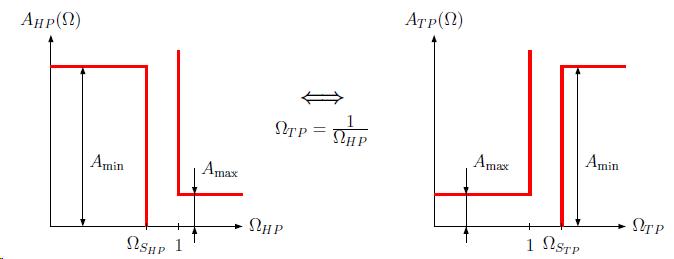
\includegraphics[width=\columnwidth]{Images/hptp}
\end{center}
Desweiteren müssen $\Omega_{S_{TP}} = \frac{1}{\Omega_{S_{HP}}}$ bzw. $1 = \Omega_{D_{TP}} = \frac{1}{\Omega_{D_{HP}}}$

\subsubsection{TP - BP Transofrmation}
\begin{align*}
	TP \rightarrow BP \qquad \text{bzw.} \qquad S \rightarrow \frac{S^2 + 1}{B\cdot S}
\end{align*}
Wobei $\omega_r$ die Mittelfrequenz $\omega_r = \sqrt{\omega_{B2}\cdot \omega_{B1}} =  \sqrt{\omega_{S2}\cdot \omega_{S1}}$ und $B$ der normierten Bandbreite enspricht \script{348}:
\[
B= \frac{\omega_{B2} - \omega_{B1}}{\omega_r} = \Omega_{B2} - \Omega_{B1}
\]
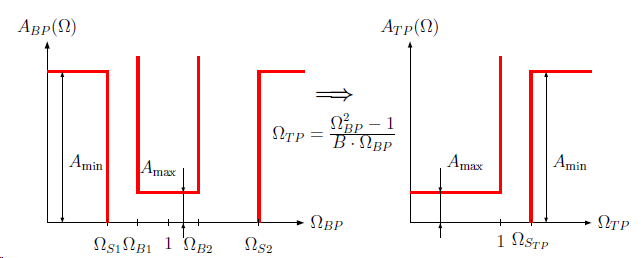
\includegraphics[width=\columnwidth]{Images/tpbp}

\subsubsection{TP - BS Transofrmation}
\begin{align*}
	TP \rightarrow BS \qquad \text{bzw.} \qquad S \rightarrow \frac{B\cdot S}{S^2 + 1}
\end{align*}
Wobei $\omega_r$ die Mittelfrequenz $\omega_r = \sqrt{\omega_{B2}\cdot \omega_{B1}} =  \sqrt{\omega_{S2}\cdot \omega_{S1}}$ und $B$ der normierten Bandbreite enspricht \script{357}:
\[
\Omega_{S_{TP}} = \frac{B}{\omega_{S2} - \omega_{S1}} = \frac{f_{B2} - f_{B1}}{f_{S2} - f_{S1}}
\]
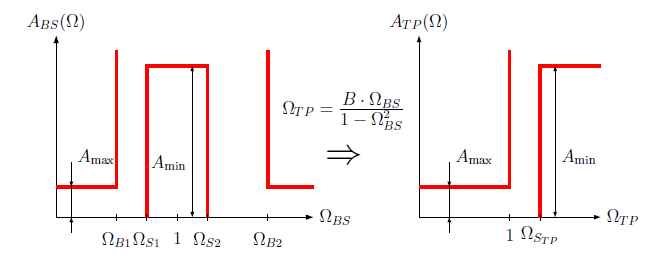
\includegraphics[width=\columnwidth]{Images/tpbs}


\subsection{LC-Netzwerke}
L und C Netzwerke haben geringste Bauteiltoleranzen. Die Struktur unterscheidet sich nicht zwischen den Filtertypen

\begin{center}
	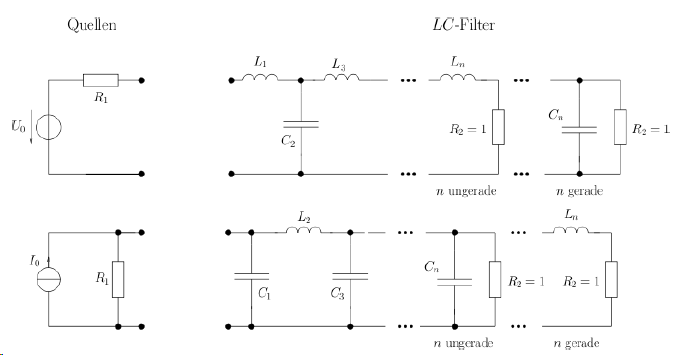
\includegraphics[width=\columnwidth]{Images/struktur}
\end{center}
